\documentclass[12pt]{article}
\usepackage[english]{babel}
\usepackage[margin=0.80in]{geometry}
\usepackage{amsmath}
\usepackage{amssymb}
\usepackage{algorithm}
\usepackage[noend]{algpseudocode}
\usepackage[utf8]{inputenc}
\usepackage{graphicx}
\usepackage{listings}
\usepackage{color}
\usepackage{hyperref}
\usepackage{cite}
%\usepackage{textcomp,uiosloforside}
\numberwithin{figure}{section}
\numberwithin{table}{section}

\definecolor{mygreen}{rgb}{0,0.6,0}
\definecolor{mymauve}{rgb}{0.58,0,0.82}
	
\lstset{
	language=Python,
	basicstyle=\footnotesize,
	commentstyle=\color{mygreen},
	keywordstyle=\color{blue},
	stringstyle=\color{mymauve},
	tabsize=4
}

\begin{document}
\begin{titlepage}
\title{Project 1 - FYS4150}
\author{Jostein Brændshøi and Trude Hjelmeland}
%\date{\today}
\date{%
    Department of Physics\\%
    University of Oslo\\[2ex]%
    \today
}
\clearpage
\maketitle
\thispagestyle{empty}

\begin{abstract}
\noindent As physicists we have encountered a fair share of differential equations and the applications of such equations remain a large motivation for projects like this. Only a handful have analytical solutions, so numerical approximations are often needed. In this project we have familiarized us with C++ as a programming language through solving the one-dimensional Poisson equation with Dirichlet boundary conditions by rewriting it as a set of linear equations. More specifically, a linear algebra problem involving a tridiagonal matrix. Since we are in the lucky position that there exists an analytical closed-form solution to the problem at hand, we have been able to focus on numerical precision as well as algorithm performance and getting to know C++ in general. Here we have found that our numerical approximation converges with the exact solutions at a fairly rapid pace and that there is a limit on how small we can make the step size before loss of numerical precision start dominating our approximation. However until this limit is reached we shall see that the error is of order grid spacing squared corresponding with the mathematical truncation error.
\end{abstract}
\vspace{2.00cm}

\noindent The address \url{https://github.com/jostbr/FYS4150-Projects/tree/master/Project1} on Git-Hub is associated with this project. Here one can find all code used in the project. This includes a main C++ source file containing the core of the project, but also Python plotting scripts for result visualization. Most of the Python scripts are fairly simple and uninteresting, but in the script for visualizing the relative error, there is some more code that might be of interest in order to see how we extracted the maximum relative error. One can also find some benchmark results as well as \LaTeX \ source for this PDF.

\end{titlepage}
\pagebreak

%\noindent Regarding the structure of this report: We will start with some introductory words on the problem, then describe and derive the methods we've employed. Futhermore there's some discussion regarding the performance of the various methods used. Finally we present the results of our numerical computations both in the context of comparing with the analytial solution, but also through examining the error of our approximation and how it evolves depending on the problem size.

% ========================================================================================
% ========================================================================================
\section{Introduction}
In this project we have examined tridiagonal matrices and developed a C++ code for numerically solving sets of linear equations represented by such matrices. The general solver which we have adopted here is known as Thomas algorithm \cite{ThomasAlg}. This is a simplified version of Gaussian elimination and greatly reduce the number of floating point operations (FLOP) needed to solve a set of equations, that can be represented by a tridiagonal matrix system on the form $\mathbf{A}\mathbf{v} = \mathbf{g}$, from  $\mathcal{O}(n^3)$ for standard Gaussian elimination to $\mathcal{O}(n)$. That being said, solving linear systems isn't the only aim of this project. Part of our motivation for developing the tridiagonal solver is to use it as a tool for solving the 1D Poisson equation stated below. We are also concerned with algorithm efficiency and performance as well as numerical precision and errors.\\

\noindent First we will present the mathematical problem we are about to solve numerically along with it's known analytical solution. We move on by presenting the discretization of the differential equation and how the mathematical operations, needed to solve this manually for a small matrix, give us the set up for the algorithms we employ. Then we discuss the algorithms performance in terms of FLOP and CPU time, before we move on to presenting the results for our numerical approximation. The relative error found between the exact and our numerical solution is discussed in the context of numerical precision. Finally we end with a broader conclusive overview. 				\\


% ========================================================================================
% ========================================================================================
\section{Methods}

\subsection{The problem at hand}
\noindent The one-dimensional Poisson equation is given as;

\begin{equation}
-u''(x) = f(x) \label{poisson1d}
\end{equation}

\noindent We want to solve this equation numerically in the interval; $x\in(0,1)$, and apply the boundary conditions that  $u(0) = u(1) = 0$.\\

\noindent We have used $f(x)=100e^{-10x}$ as a source term which gives us that the analytical solution to the problem is:
\begin{equation}
u(x) =1 - (1-e^{-10})x - e^{-10x} \label{analytical}
\end{equation}

\noindent By substituting equation \eqref{analytical} into \eqref{poisson1d} we see that equation \eqref{analytical} is in fact the analytical solution to the one-dimensional Poisson equation when we have $f(x)=100e^{-10x}$ and we will use this fact in our analysis of the numerical precision of our approximation. Below we attempt to solve this problem numerically using linear algebra and simple algorithms. \\

% ========================================================================================
% ========================================================================================

\subsection{Discretization and matrix setup}
We approximate the second derivative of $u$ with a common centered finite difference for solving differential equations, the three point formula, given as:

\begin{equation}
   v_i'' = \frac{v_{i+1}+v_{i-1}-2v_i}{h^2} + \mathcal{O}(h^2)    \hspace{0.5cm} \mathrm{for} \hspace{0.2cm} i=1,\dots, n, \label{discretization}
\end{equation}

\noindent where $v_i=v(x_i)$ and $\mathcal{O}(h^2)$ is the truncation error, which we will come back to when we talk about numerical precision. Equation (3) can be derived using Taylor series. In this project we have discretized the approximation for $u$ as $v$ in the interval from $x_0=0$ and $x_{n+1}=1$ with the grid points $x_i=ih$ where $h$ is defined as $h=\frac{1}{n+1}$ and defines the grid spacing. When using (3) as a an approximation to the left-hand-side in (1), it is possible to rewrite (1) as a set of linear equations on the form: 

\begin{equation}
	\label{matrixeq}
   \mathbf{A}\mathbf{v} = \mathbf{g},
\end{equation}

\noindent where $v_i$ is the numerical solution we seek, $g_i=h^2f_i$, $f_i$ is the source function at $x_i$ and $\mathbf{A}$ is an $n\times n$ tridiagonal matrix coming from the discretization of the second order derivative given as:

\begin{equation}
    \mathbf{A} = \begin{bmatrix}
                           2& -1& 0 &\dots   & \dots &0 \\
                           -1 & 2 & -1 &0 &\dots &\dots \\
                           0&-1 &2 & -1 & 0 & \dots \\
                           & \dots   & \dots &\dots   &\dots & \dots \\
                           0&\dots   &  &-1 &2& -1 \\
                           0&\dots    &  & 0  &-1 & 2 \\
                      \end{bmatrix} \label{matrixA}
\end{equation}




\noindent Here we recognize the coefficients of equation \eqref{discretization} as the upper-, lower- and diagonal elements of matrix $\mathbf{A}$ with a sign change which follows from how the Poisson equation (1) is defined. A tridiagonal matrix is a special type of banded matrix where all other elements then the elements directly below and over the leading diagonal i zero, leading to the condition that the matrix is tridiagonal if $a_{ij}=0$ for $|i-j|>1$ and all diagonal elements are nonzero.\\

\noindent We noe attempt to show that \eqref{poisson1d} can be written as \eqref{matrixeq}. Insert \eqref{discretization} (but neglect the $\mathcal{O})h^2)$ term) for $u$ in \eqref{poisson1d} and multiply with $h^2$ to get

\begin{equation}
	\label{General}
 2v_i - v_{i+1} - v_{i-1} = h^2 f_i = g_i
\end{equation}

\noindent To investigate further lets look at specific values of index $i$:

\begin{align*}
i=1: & \hspace{0.5cm} 2v_1 - v_{2} - v_{0} = g_1 & 					\\
i=2: &	\hspace{0.5cm} 2v_2 - v_{3} - v_{1} = g_2 & 					\\
i=3: &	\hspace{0.5cm} 2v_3 - v_{4} - v_{2} = g_3 & 					\\
\vdots & \hspace{1.5cm} \vdots	&			\\
i=n: & \hspace{0.5cm} 2v_n - v_{n+1} - v_{n-1} = g_n & 
\end{align*}

\noindent and now rewrite this in terms of scalar products (of two vectors) on the left-hand-side:

\begin{align*}
i=1: & \hspace{0.5cm} (2, -1, 0 \dots ,0)\cdot(v_1, \dots , v_n) = g_1 & 					\\
i=2: & \hspace{0.5cm} (-1, 2, -1, 0 \dots ,0)\cdot(v_1, \dots , v_n) = g_2 & 					\\
i=3: & \hspace{0.5cm} (0, -1, 2, -1, 0 \dots ,0)\cdot(v_1, \dots , v_n) = g_3 & 					\\
\vdots &	\hspace{1.5cm}		\vdots																\\
i=n: & \hspace{0.5cm} (0, \dots -1, 2)\cdot(v_1, \dots , v_n) = g_n & 					\\
\end{align*}

\noindent (remember $v_0=v_{n+1}=0$ from the boundary conditions). We now see that each element $g_i$ in $\mathbf{g}$ is computed through a scalar product corresponding with the definition of how matrix-vector mutliplications are calculated. This leads to the conclusion that each of left vectors on the left-hand-sides for the various $i$-cases make up the matrix $\mathbf{A}$ which corresponds with the one seen in \eqref{matrixA}. Also, the way we defined $\mathbf{v}$ and $\mathbf{g}$ corresponds with \eqref{matrixeq} and thus \eqref{poisson1d} can be rewritten as \eqref{matrixeq}. Knowing this we can start looking at some algorithms for solving \eqref{matrixeq}, which is the aim for the next two subsections.


% ========================================================================================
% ========================================================================================
\subsection{Gauss elimination for general tridiagonal matrix} \label{sec:genalgsection}
% Some algorithm stuff
We can write out $\mathbf{A}\mathbf{x} = \mathbf{y}$ for a general tridiagonal matrix $\mathbf{A}$

\[
    \begin{pmatrix}
                           b_1& c_1& 0 &\dots   & \dots &0 \\
                           a_1 & b_2 & c_2 &0 &\dots &\dots \\
                           0& a_2 & b_3 & c_3 & 0 & \dots \\
                           & \dots   & \dots &\dots   &\dots & \dots \\
                           0&\dots   &  & a_{n-2} & b_{n-1}& c_{n-1} \\
                           0&\dots    &  & 0  & a_{n-1} & b_n \\
    \end{pmatrix}
    \begin{pmatrix}
    x_1 \\ 
    x_2 \\
    \vdots \\
    x_n \\
    \end{pmatrix}
    =
    \begin{pmatrix}
    y_1 \\
    y_2 \\
    \vdots \\
    y_n\\
    \end{pmatrix}
\] 

\noindent The equivalent set of linear equations reads then:

\begin{equation}
a_i v_{i-1} + b_i v_i + c_i v_{i+1} = f_i \hspace{0.5cm} \mbox{for} \hspace{0.2cm} i = 1 \dots n \label{linearalg}
\end{equation}

\noindent To make sure that the matrix $\mathbf{A}$ yields solutions to the set of linear equations we can look for weak dominance of diagonal elements which is fulfilled when the conditions $|b_1| > |c_1|$, $|b_n| > |a_n|$ and $|b_j|\geqslant |a_j| + |c_j|$ for $j=2, 3 \dots n-1$ are met. In addition the matrix $\mathbf{A}$ must be irreducible, which means that $a_i$ and $c_i$ are non-zero elements. \cite{Comp} With a quick glans at the matrix $\mathbf{A}$ defined by our problem and given in the introductions, it is straight forward to see that the two above mentioned conditions are met in our case.
\vspace{0.35cm}

\noindent To arrive at an general algorithm for solving the set of linear equations defined by a tridiagonal matrix, lets consider the following example. Here we will not assume that the matrix elements $a_i$ are equal to $c_i$ and for simplicity we derive this for a matrix $\mathbf{A}\in \mathbb{R}^{4\times4}$.

\[
    \begin{pmatrix}
                           b_1& c_1& 0 &0 \\
                           a_1 & b_2 & c_2 &0 \\
                           0& a_2 & b_3 & c_3 \\
                           0& 0& a_3 & b_4                         \\
                           
    \end{pmatrix}
    \begin{pmatrix}
    x_1 \\ 
    x_2 \\
    x_3 \\
    x_4 \\
    \end{pmatrix}
    =
    \begin{pmatrix}
    y_1 \\
    y_2 \\
    y_3\\
    y_4\\
    \end{pmatrix}
\] 

\noindent This leads to the set of linear equations:

\begin{align*}
b_1 x_1 + c_1 x_2 + 0 + 0 = y_1 \\
a_1 x_1 + b_2 x_2 + c_2 x_3 + 0 = y_2 \\
0 + a_2 x_2 + b_3 x_3 + c_3 x_4 = y_3 \\
0 + 0 + a_3 x_3 + b_4 x_4 = y_4\\
\end{align*}

\noindent For simplicity we will now leave out all the $x_i$ values in the further derivation of the algorithm. We apply Gaussian elimination where we subtract line number one from line number two after multiplying line one with a fitting constant that helps us eliminate the first element of line two. In our case we multiply line one with $\frac{a_1}{b_1}$ and subtract from line two giving us:

\begin{align*}
b_1 + c_1  + 0 + 0 = y_1 \\
0 + (b_2 - \frac{a_1 c_1}{b_1}) + c_2 + 0 = (y_2 - \frac{y_1 a_1}{b_1}) \\
0 + a_2 + b_3 + c_3 = y_3 \\
0 + 0 + a_3 + b_4 = y_4\\
\end{align*}

\noindent We now rename the two expressions in the brackets for $\tilde{b_2}$ and $\tilde{y_2}$ respectively. When we preform the same operation on the next two lines we end up with:

\begin{align*}
b_1 + c_1  + 0 + 0 = y_1 \\
0 + \tilde{b_2} + c_2 + 0 = \tilde{y_2} \\
0 + 0 + \tilde{b_3} + c_3 = \tilde{y_3} \\
0 + 0 + 0 + \tilde{b_4} = \tilde{y_4} \\
\end{align*}

\noindent where $\tilde{b}_3= b_3 - \frac{a_2 c_2}{\tilde{b_2}}$ and $\tilde{b}_4= b_4 - \frac{a_3 c_3}{\tilde{b_3}}$. Likewise $\tilde{y_3} = y_3 - \tilde{y_2} \frac{a_2}{\tilde{b_2}}$ and $\tilde{y_4} = y_4 - \tilde{y_3} \frac{a_3}{\tilde{b_3}}$ and thus we see that we can generalize this to

\begin{equation}
 \tilde{b}_i= b_i - \frac{a_{i-1} c_{i-1}}{\tilde{b_{i-1}}} \label{genbi}
\end{equation}

\begin{equation}
\tilde{y_i} = y_i - \tilde{y_{i-1}} \frac{a_{i-1}}{\tilde{b_{i-1}}} \label{genyi}
\end{equation}

\begin{algorithm}
\caption{General tridiagonal matrix algorithm}\label{alg:tridiaggen}
\begin{algorithmic}[1]
\Procedure{tridiag\_gen}{}
	\State $\tilde{b}_0=b_0$ \qquad// First element along main diagonal
    \State $\tilde{y}_0=y_0$ \qquad// First element in right side of equation\\
	\For {$i=1$ to $i=N-1$}
		\State $\tilde{b}_i=b_i-a_{i-1}*c_{i-1}/\tilde{b}_{i-1}$		  \qquad// Eliminate lower diag
		\State $\tilde{y}_i=y_i-a_{i-1}*\tilde{y}_{i-1}/\tilde{b}_{i-1}$  \qquad// Change right side
	\EndFor \\
    
    \State $x_{N-1}=\tilde{y}_{N-1}/\tilde{b}_{N-1}$ \qquad\qquad// Final element in solution\\
    
    \For {$i=N-2$ to $i=0$}
		\State $\tilde{v}_i=(\tilde{y}_{i}-c_i*v_{i+1})/\tilde{b}_i$ \qquad// Find all other elements of sol.
	\EndFor \\
    
    \State \Return($v$)
\EndProcedure
\end{algorithmic}
\end{algorithm}

\noindent Now we see that the last line in the equation set over is uncoupled from the rest of the system, giving us that $ \tilde{y_4} = \tilde{b_4} x_4$. This allows us to do a backward substitution by inserting in the value of $x_4 = \frac{\tilde{y_4}}{\tilde{b_4}}$ into the equation for $x_3$ on the second last line. This gives $x_3=(\tilde{y}_3-c_3x_4)/\tilde{b}_3$ which we generalize as:

\begin{equation}
 x_i = \frac{\tilde{y_i} - c_i x_{i+1}}{\tilde{b_i}} \label{genxi}
\end{equation}

\noindent This leads us to solving the equation set defined by a tridiagonal matrix by two easy steps; a forward substitution to eliminate the lower diagonal elements and a backward substitution to eliminate the upper digonal elements and obtain $x_i$, given that the matrix is weak diagonal dominant and irreducible \cite{Comp}. When implementing \eqref{genbi}, \eqref{genyi} and \eqref{genxi} we have to consider the fact that C++ indices's starts at zero. This slightly alters the indexing of the formulas and pseudo code for the computer implementation is shown in Algorithm \ref{alg:tridiaggen}.

%May include something about how we can test for this in the general case. 

% ========================================================================================
% ========================================================================================
\subsection{Gauss elimination for simplified tridiagonal matrix}
While it's interesting and informative to look at the general case as discussed in section \ref{sec:genalgsection}, it's worthwhile trying to further exploit the form of matrix $\mathbf{A}$, as displayed in \eqref{matrixA}, to obtain a more efficient algorithm. If we use the fact that $a_i=c_i=-1$ and $b_i=2$, then line 3 in algorithm \ref{alg:tridiaggen} evolves as

\begin{align}
	\tilde{b}_i&=b_i-a_{i-1}c_{i-1}/\tilde{b}_{i-1} \nonumber \\
    \tilde{b}_i&=b_i-1/\tilde{b}_{i-1} \nonumber \\
    &\hspace{1cm}\vdots \nonumber \\
    \tilde{b}_2&=2-1/2=3/2 \nonumber \\
    \tilde{b}_3&=2-2/3=4/3 \nonumber \\
    \tilde{b}_4&=2-3/4=5/4 \nonumber \\
    &\hspace{1cm}\vdots \nonumber \\
    \tilde{b}_i&=(i+1)/i \ , \qquad i=2,\dots,n \label{simpleb}
\end{align}

\noindent where $\tilde{b}_1=b_1=2$ (this could also technically be captured by equation \eqref{simpleb}, but is left out as $\tilde{b}$ is properly well defined starting from the second row in the matrix). As with the general algorithm above, we have to slightly alter the indexing when implementing the specialized algorithm. Starting with Algorithm \ref{alg:tridiaggen} and using $a_i=c_i=-1$ and $b_i=2$ (leading to equation \eqref{simpleb} and other small simplifications) yields Algorithm \ref{alg:tridiagspe}.
\pagebreak

\begin{algorithm}
\caption{Specialized tridiagonal matrix algorithm}\label{alg:tridiagspe}
\begin{algorithmic}[1]
\Procedure{tridiag\_spe}{}
	\State $\tilde{b}_0=2$ \ \qquad// First element along main diagonal
    \State $\tilde{y}_0=y_0$ \qquad// First element in right side of equation\\\\
    
	\For {$i=1$ to $i=N-1$}
		\State $\tilde{b}_i=(i+2)/(i+1)$						 \qquad// Eliminate lower diag
		\State $\tilde{y}_i=y_i+\tilde{y}_{i-1}/\tilde{d}_{i-1}$ \qquad// Change right side
	\EndFor \\
    
    \State $x_{N-1}=\tilde{y}_{N-1}/\tilde{d}_{N-1}$ \qquad\qquad// Final element in solution\\\\
    
    \For {$i=N-2$ to $i=0$}
		\State $\tilde{v}_i=(\tilde{y}_{i}-v_{i+1})/\tilde{d}_i$ \qquad // Find all other elements of sol.
	\EndFor \\
    
    \State \Return($v$)
\EndProcedure
\end{algorithmic}
\end{algorithm}


% ========================================================================================
% ========================================================================================



\section{Results}

\subsection{Algorithm performance}
\noindent Regarding floating-point operations (FLOP), we can count these by looking at the algorithms. Starting with the general algorithm we have, for the forward substitution, 3 floating-point operations to compute $\tilde{b}_i$ and 3 to compute $\tilde{y}_i$ This is repeated for $N-1$ iterations resulting in $6(N-1)$ FLOP. Then for the backward substitution step, we have again 3 FLOP repeated $N-1$ times in addition to 1 FLOP for the upper edge point in the solution. In total these combine to (refer to pseudo code above for $N$)
\begin{equation*}
	\text{FLOP}_{gen}=3(N-1)+3(N-1)+1+3(N-1)=9(N-1)+1
\end{equation*}
These are just the total number of floating-point operations done in the algorithm. If we would like to know the more commonly used term, FLOPS (floating-point operations per second), we would divide $9(N-1)+1$ by the CPU time used by the algorithm. This can be done for various problem sizes (different $N$'s) and is illustrated in Table \ref{CPU}.
\vspace{0.35cm}

\noindent For the specialized algorithm we can count similarly, however, we see that we have reduced the number of FLOP. To compute $\tilde{b}_i$ we only need 1 FLOP (as opposed to 3) as seen in $(i+2)/(i+1)$ (we don't count integer operations in the numerator and denominator, only the floating point division). Due to the lower diagonal elements being all equal to 1, we only need 2 FLOP to compute $\tilde{y}_i$ meaning we save 1 FLOP here. Similarly, we need 2 FLOP to compute $v_i$ since also all the upper diagonal elements are equal to 1. The upper edge point $v_N$ still require 1 FLOP and the number of iterations are the same as in the general case. Combining the above, the specialized algorithm require

\begin{equation*}
	\text{FLOP}_{spe}=1(N-1)+2(N-1)+1+2(N-1)=5(N-1)+1
\end{equation*}

\noindent It could now be interesting to compare the to FLOP results. Assuming $N$ is large, we can write

\begin{equation*}
\frac{\text{FLOP}_{gen}}{\text{FLOP}_{spe}}=\frac{9(N-1)+1}{5(N-1)+1}=\frac{9(N-1)}{5(N-1)+1}+\frac{1}{5(N-1)+1}\approx\frac{9(N-1)}{5(N-1)}=\frac{9}{5}=1.8
\end{equation*}

\noindent Based on this, it seems like the specialized algorithm contains almost half the floating-point operations. this would lead us to expect that, for sufficiently large $N$, the specialized algorithm would perform around 80\% faster than the general. However this is not the case as seen in Table \ref{CPU}. Why? It's not a straightforward question to answer, but one can for example consider the simplifications done when dealing with FLOP. For instance the simplified version needs fewer FLOP, but in \eqref{simpleb} (and the other lines in Algorithm \ref{alg:tridiagspe}) we still have the float division, meaning we've got rid of some FLOP, but limited to addition and multiplication. And with division being the most computationally expensive floating-point operation, this can therefore be part of the reason why we're not seeing in table \ref{CPU} as large of a speedup as we would expect. \\

\begin{table}[ht]
%\caption{Timing our code}
\begin{center}
\label{CPU}
  \begin{tabular}{| l | l | l | l |}
  \hline
    Number, $N$ &  Generalized [s] & Special [s] & Armadillo [s]\\[0.10cm]\hline\hline
     & & & \\
     10 & $3.6\cdot10^{-6}$ & $4.2\cdot10^{-7}$ & $1.3\cdot10^{-5}$\\[0.10cm]
    100 & $2.4\cdot10^{-6}$ & $2.3\cdot10^{-6}$& $5.7\cdot10^{-4}$\\[0.10cm]
     1000 & $2.8\cdot10^{-5}$& $2.5\cdot10^{-5}$& $2.9\cdot10^{-1}$\\[0.10cm]
     \hline
  \end{tabular}
\end{center}
\caption{Comparing CPU time for the three different algorithms utilized in this project. The number $N$ defines the size of the $n\times n$ matrix we solve. All times are averaged over 100 runs for the different algorithms and matrix sizes to obtain higher accuracy of the timing. Also see figure 3.1 for a more visual representation.}
\end{table}

\begin{figure}[ht]
\label{runtime}
\centerline{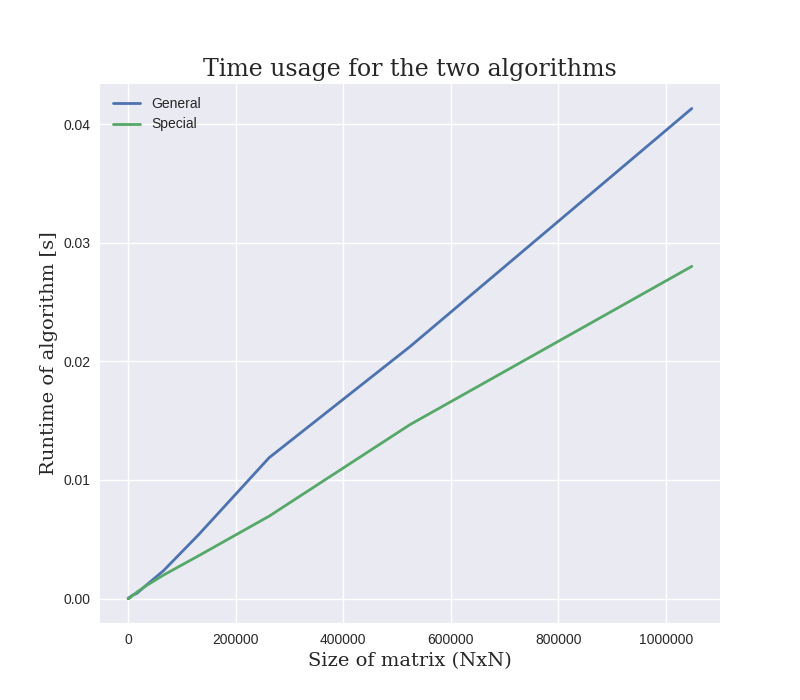
\includegraphics[scale=0.7]{runtime_comparison.png}}
	\caption{A plot comparing the runtime for our two algorithms as function of matrix size. Her we see that the benefit of utilizing our specialized algorithm get more pronounced as the matrix size increases. This is due to the to graphs having different slopes. Although note the straight form of the graphs, indicating that runtime is a linear function of the problem size $n$ as discussed above for both algorithms.}
\end{figure}

\noindent As a third alternative we have written some code that utilizes the built in functions found in the Armadillo library\cite{Arma} for solving sets of linear equations with the function \texttt{arma::solve()}. In contrast to the standard Gaussian elimination Armadillo preforms an LU decomposition of our matrix $\mathbf{A}$ first and then solves it by forward and backward substitution (similar to that used in the tridiagonal algorithm). Armadillo will still solve this for any square matrix so in our case where we are dealing with an matrix which only contains nonzero elements along the upper-, lower- and diagonal elements Armadillo will preform the same operations on all the zero elements in our matrix. In our case this is clearly not needed and significantly increases the CPU time when our matrix starts exceeding $N=10$ in comparison to our two specialized algorithms whom utilizes the fact that we are solving the problem for a tridiagonal matrix. The unattention to the fact that we have a tridiagonal matrix leads the LU-decomposition to require $\mathcal{O}(n^3)$ FLOP which is reflected in the far longer runtime in table \ref{CPU} \cite{Comp}. Another issue is memory usage. The general LU-decomposition algorithm requires us to store the entire matrix $\mathbf{A}$ in memory which significantly limits the number of grid points we can use in the computations. For instance attempting with $n=10^5$ implies a $10^5\cdot10^5=10^{10}$ matrix to be stored in memory. This equates to $10^{10}*64/(8\cdot 10^9)=80$GB of memory assuming use of double precision numbers. This is far past the limit of the normal amount of memory (around 8GB) available on personal computers. Hence using the general LU-decomposition algorithm for this matrix size will not work on our machines.

% ========================================================================================
% ========================================================================================

\subsection{Numerical solution and testing}

\noindent The main objective of this project have been to numerically approximate the one dimensional Poisson equation using finite differences resulting in a tridiagonal matrix $\mathbf{A}$ and linear algebra problem $\mathbf{A} \mathbf{v} = \mathbf{g}$. As we have seen this results in a simple algorithm where we preform forward- and backwards substitution to approximate the solution. For the sake of clarity we have limited our self to only present the results for our specialized algorithm (the general produces the same results). In figure \ref{fig:result} we see that our numerical solution converges with the exact one to a great extent already for $n=100$. So the algorithm seem produce expected results. An more detailed discussion on the relative error between our numerical- and analytical solution can be found in section \ref{sec:numprec}.\\ 


\begin{figure}[ht]
\label{fig:result}
\centerline{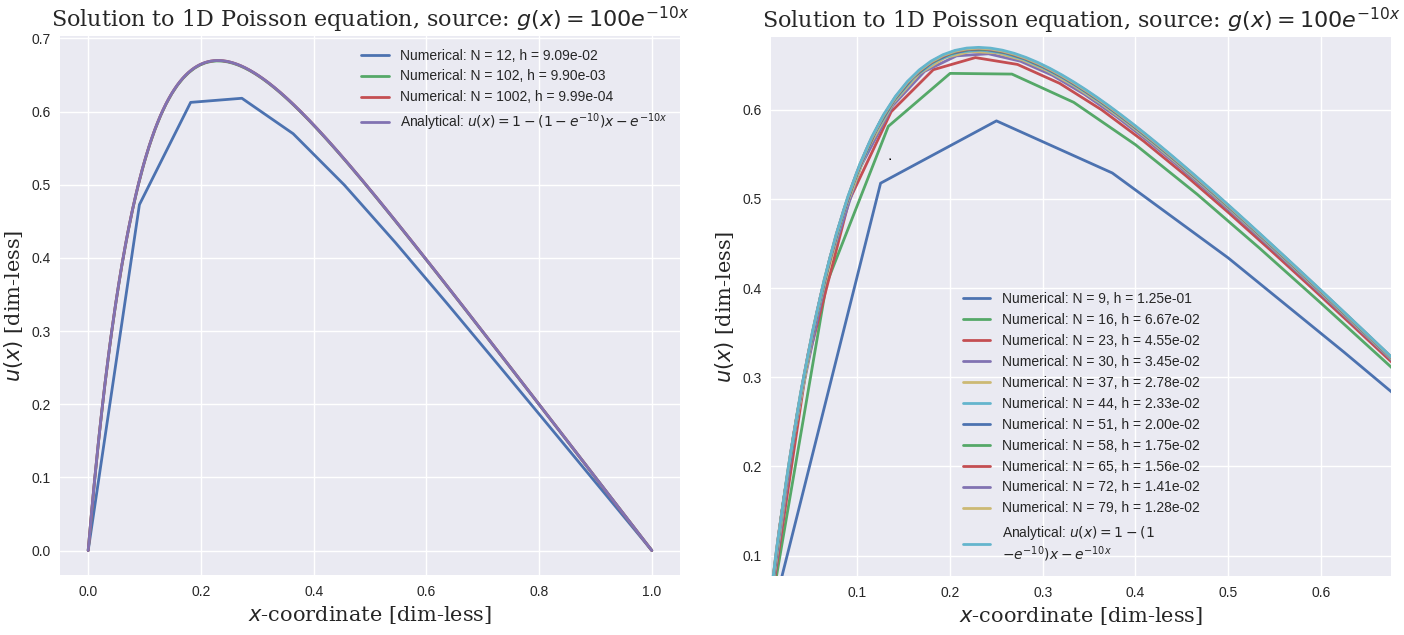
\includegraphics[scale=0.47]{double_illustration.png}}
	\caption{Plots of the numerical approximation and the exact solution to the 1D Poisson equation for different values n, which define the $n \times n$ matrix size, for our special tridiagonal matrix where the upper- and lower diagonal elements are all equal to -1. Plot to the right is included to show how fast the approximated solutions converges with the exact one as n is increased towards 80. }
\end{figure}

\noindent We have benchmarked our code by saving selected numerical results in a benchmark folder on GitHub. To replicate these results you need to pass the arguments 10 100 1000, to set up the matrix sizes we want to solve for, on the command line when running \texttt{tridiag.cpp}. Also there are benchmark results for timing of the three algorithms (data in figure \ref{runtime}). To replicate these, one calls \texttt{benchmark("general", 23, 5)}, \texttt{benchmark("special", 23, 100)} (while changing the base number, within \texttt{benchmark()} from 10 to 2). \\

\noindent In addition to testing the code up against the analytical solution \eqref{analytical}, we have also created a unit test for the generalized tridiagonal solver, which tests if $\mathbf{A}\mathbf{x}=\mathbf{y}$, with given $\mathbf{A}$ and $\mathbf{y}$ results in the expected $\mathbf{x}$ that we have computed by hand on paper. We have found the correct values by analytically solving the problem for a $3 \times 3$ matrix We have used
\begin{equation}
    \mathbf{A} = \begin{bmatrix}
                           1 & 1 & 0 \\
                           1 & 2 & 1 \\
                           0 & 1 & 3 \\
                      \end{bmatrix}
                      \ , \qquad \mathbf{y}=\begin{bmatrix}
                           -1 \\
                           -1 \\
                           -1 \\
                      \end{bmatrix}
\end{equation}

\noindent which gives the solution $\mathbf{x}=[x_1, x_2, x_3]=[-1.5, 0.5, -0.5]$. The unit test compares the known solution to the numerical solution and if these are the same a message will be prompt in the terminal window telling the user that the test is passed. However, if the values don't correspond the test has failed and the user is notified. One advantage with using such a test is that, during development, if one make changes to the algorithm, one can immediately see if the changes resulted in unwanted behavior through running the test. This can save time during development. \\

%-----------------------------------------------------------------------------------
%-----------------------------------------------------------------------------------
\subsection{Numerical precision} \label{sec:numprec}

\noindent As mentioned earlier, we introduce a truncation error when we use equation \eqref{discretization} to approximate the second derivative. The truncation error occurs because we reduce a Taylor expansion to only a few number of terms instead of including the whole series. It is possible to predict the extent of the truncation error and in our case we expect this to go like $\mathcal{O}(h^2)$. We will use this fact in our further analysis of the numerical precision.  \\

\noindent An important source of error in the numerical approximation is round off errors which arises from the fact that computer can not represent all numbers accurately and these need to be rounded off to a number the computer can represent. This round off is dependent on the number of bites we use to represent the number and how many significant digits we use. We have used double precision meaning that computer uses 8 bytes to represent a number. \\

\noindent In our case, the system of equation that we are solving numerically have an analytical solution. So a great way to get an impression of our numerical precision is to calculate the relative error $\epsilon_i$ (at grid point $x_i$) between the numerical solution, $v_i$, and the analytical solution, $u_i$, in each grid point:

\begin{equation}
\label{RelErr}
 \epsilon_i = log_{10} \left(\frac{|v_i - u_i|}{|u_i|}\right)
\end{equation}

\begin{table}[ht]
\begin{center}
\label{RelativErr}
  \begin{tabular}{| l | l |}
  \hline
    Number, $N$ &  Relative error (log10)  \\[0.10cm]\hline \hline
     & \\
     10 & $  -1.18  $  \\[0.10cm]
     100 & $  -3.09 $  \\[0.10cm]
     1000 & $  -5.08 $ \\[0.10cm]
     10 000 & $ -7.08  $ \\[0.10cm]
     100 000 & $ -9.08  $ \\[0.10cm]
     1 000 000 & $  -10.16  $ \\[0.10cm]
     10 000 000 & $ -9.09	$			\\[0.1cm]
     \hline
  \end{tabular}
\end{center}
\caption{Compare the relative error, as defined in equation \eqref{RelErr}, for different $n$ values which defines the $n \times n$ matrix size for the specialized algorithm. Here we have calculated the relative error for each grid point and then extracted the maximum value for the relative error for each value of $n$. Here the relative errors are listed in a logarithmic scale.}
\end{table}

\noindent If the relative error, defined as above, should follow the truncation error $\mathcal{O}(h^2)=\mathcal{O}(1/n^2)$, we should expect the relative error to decrease by about a factor 100 for every increase by a factor 10 in grid points. In our table \ref{RelativErr} and figure \ref{fig:relerr} we have chosen to focus on the relative error as a function of $n$ instead of $h$ as we found this to be a slightly more intuitive approach. We can see from table \ref{RelativErr} (recall that the error here is on a logarithmic scale) and figure \ref{fig:relerr} that our expectations are met up to a point of $n=10^5$. Here the error follows the mathematical truncation error $\mathcal{O}(h^2)=\mathcal{O}(1/n^2)$. Then the behavior of the relative error starts deviate from the relation predicted for the truncation error. From $n=10^5$ we see an decrease in the slope towards $n=10^6$ before the relative error starts increasing as $n$ increases towards $10^7$. This seems to be where round off error starts dominating the precision of our numerical approximation. This means that we can not let $h \to 0$ without loss of numerical precision.  \\


\begin{figure}[ht]
	\label{fig:relerr}
	\centerline{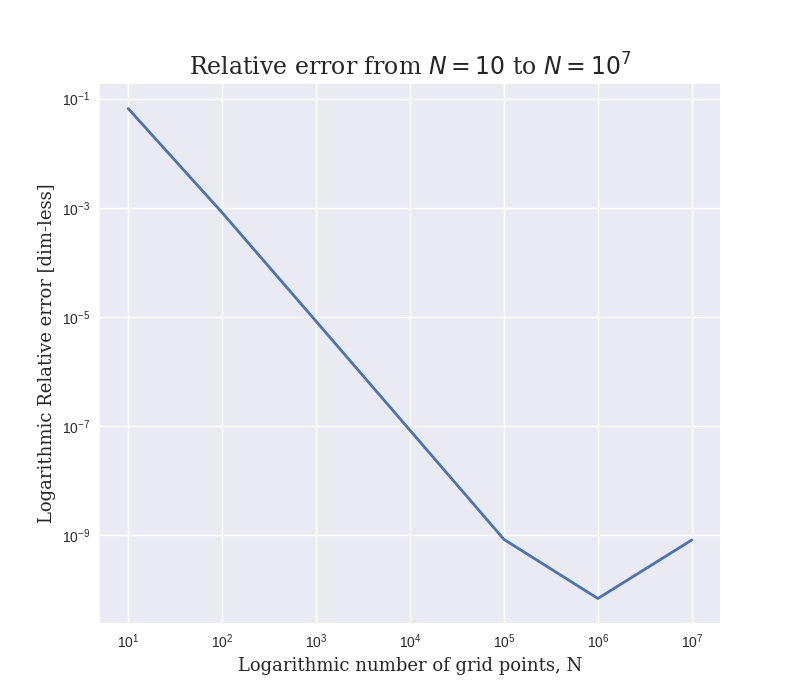
\includegraphics[scale = 0.70]{relative_error.png}}
	\caption{A plot of the relative error, as defined in \eqref{RelErr}, as a function of the grid points $n$. Here we can see that the relative error follows our expectation for the truncation error, with a slope value of -2 on a logarithmic scale, up to a point of $n\sim 10^5$.}
\end{figure}

%====================================================================================
%
%====================================================================================

\section{Concluding remarks}
\noindent In this project we have looked at numerical applications of linear algebra to the solution of the 1D Poisson equation. For this context we've written C++ code to implement algorithms for solving a set of linear equations represented by a tridiagonal matrix. We have found that the different algorithms perform at various speeds and that our numerical approximation converges with the exact solution to a great extent already for $n=10^2$, but also that it is not possible to let the grid spacing $h \to 0$ with out the loss of numerical precision. We have also compared \\

\noindent There are many possible solutions to solve our problem numerically. Standard Gaussian elimination is the brute force approach which can solve our problem for any square matrix but this requires many FLOPs and is excessive to use in our case with a tridiagonal matrix where all other elements except the three diagonals are zero. Another approach to standard Gaussian elimination have been made by utilizing Armadillos built in function \texttt{arma::solve()}. This function preforms an LU decomposition of the matrix $\mathbf{A}$ before using Gauss elimination and also performs unecessary many oprations resulting in $\mathcal{O}(n^3)$ FLOP. We can not utilize this function for big matrices and we have seen that already for a matrix size of $n=10^5$, our computer runs out of memory. Advantages of this method consists of it being able to solve for an arbitrary matrix and that, if there are any zero elements along the diagonal, the command solve() will automatically perform pivoting. This is not the case for our general tridiagonal solver which would fail (due to zero division) if some of the elements along main diognal were zero. \\

\noindent To improve on the Armadillo algorithm, we have taken advantage of the fact that we are dealing with a tridiagonal matrix and developed an general tridiagonal solver. This reduces the required FLOP to $\sim 9n$ giving our algorithm a clear advantage in terms of CPU time and solvable matrix sizes, but our algorithm is of course limited to the case with, although general, a tridiagonal matrix $\mathbf{A}$. We have also developed an algorithm that only solves our problem for the specified tridiagonal matrix \eqref{matrixA}, where all elements are 2 along the diagonal and -1 along the upper- and lower diagonal. This further reduces the required FLOPs to $\sim 5n$ and we see from table \ref{CPU} and figure \ref{runtime} that this of course speeds up CPU time, especially for large matrices but this algorithm only functions for the special tridiagonal matrix we got from the discretization \eqref{discretization}. \\

\noindent In light of all this, a reasonable conclusion regarding the algortihms, could be that each of them have their strenghts and weaknesses and that none of the three examined are objectively better than the others. Rather they excel for each their cases and that we should choose wisely depending on the problem at hand. Considering this; for this project one would then assign the specialized algorithm as the top performer. \\

\noindent We found this project interesting and in particular we enjoyed learning some C++ for the first time. Also seeing linear algebra algorithms applied to the study of differential equations was intruiging as this is not something we have had that much on in previous courses. \\

\noindent For further enhancments to the work done, it would be possible to vectorize the statement calculating $\tilde{b}_i$ in the special case since this calculation only depend on the index value of the element i. It is then possible to put this calculation outside the main loops in the algorithm reducing the required FLOPs to $\sim 4n$.   


\bibliography{sample}{}
\bibliographystyle{plain}

\end{document}